% !TEX root = main.tex

\section{PLCによるFA制御実験}

\subsection{実験目的}
FAシステムの基礎理論であるシーケンス制御は,机上の学問や理論というより
生産現場での実務と経験が重きをなすといわれており,現場に近い状況で実際にシステムを構築することが
シーケンス制御を学習する上で最も効果的である.前回までに学んだ知識を基に本実験では,
現場に近い状況を体験するために工場などでの生産ラインを想定したFA制御実験を行う.
具体的には,磁性金属,非磁性金属,非金属の3種のワークを振り分ける制御を目標とする.

\subsection{実験装置}
本機は,3つのコンベアから構成されており,そこにセンサを取り付けることで磁性金属,
非磁性金属,非金属(それぞれ鉄・アルミ・プラスチック)を分別することを制御目的とした実験学習装置である.
上段の1段目から3段目にかけて少しずつ高低差を設けており,コンベア部には,金属センサ,アルミセンサ
,4種の光電センサを設置してある.また,図3.1に全体の配置図を示す.

\begin{figure}[h]
  \centering
  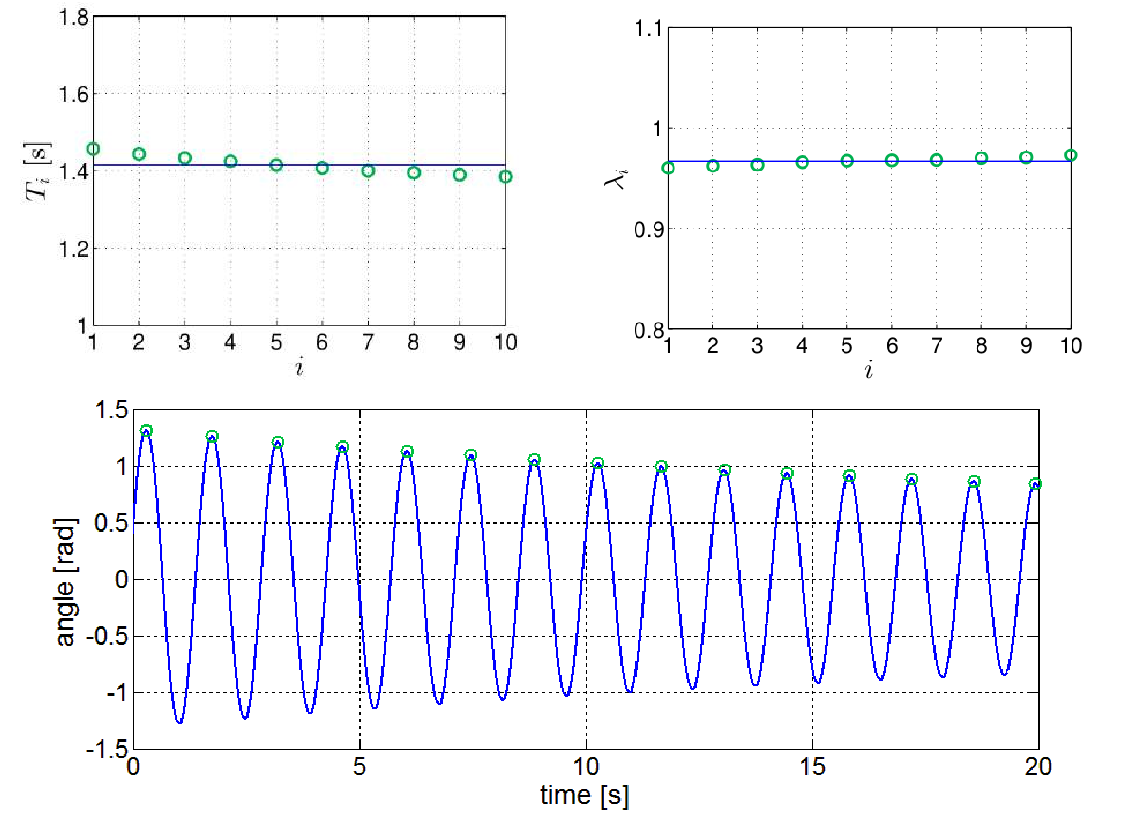
\includegraphics[width=0.5\textwidth]{sozai/6.pdf}
  \caption{全体の配置図}
\end{figure}

\subsection{モーターの配線}
図3.2に本装置に用いたインダクションモーターの配線と回転方向を示す.
これはコンデンサ接続形モーターであり,2つのコイルが内蔵されている.
その2つのコイルの片方にコンデンサを接続することで90°の位相差を生み,
運転の方向を決定している.そのため,正転・逆転の切り替えについては図示されているように,
配線を変更せずに交流100Vを使う必要がある.
本実験では,PLCで直接スイッチを行う代わりに,
耐高電流性を持つ有接点リレーを用いてモーターのスイッチングを行っている.

\begin{figure}[h]
  \centering
  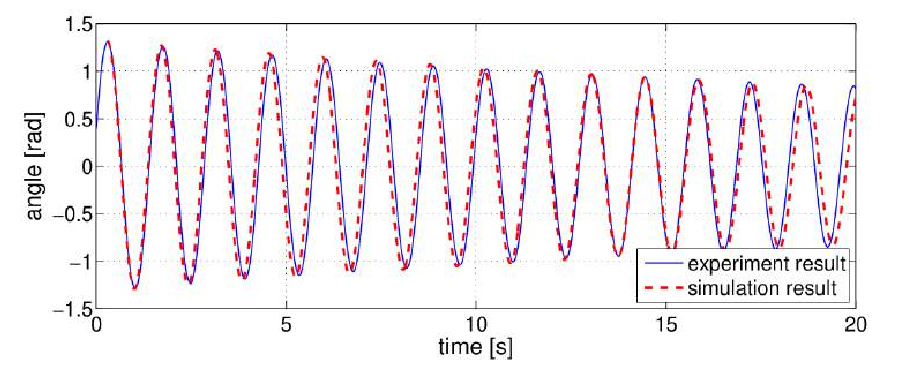
\includegraphics[width=0.5\textwidth]{sozai/7.pdf}
  \caption{モータの配線図}
\end{figure}

モーターの配線に関するより詳細な配線は図3.3~3.5に示す.
3種類の仕分対象物を,3方向に振り分ける実験装置構成が1段目は1方向だけに制御し,
2および3段目は2方向に回転方向を制御する.そのため,図3.3に示すように,
コンベア1段目ではすでに配線が決定しており,
リレー(R1)をON/OFFすればモーターをON/OFFするように構成されている.

2段目のモーター(図3.4)も基本的には同じ構成であり,
リレー(R2)をON/OFFすればモーターもON/OFFするように構成されている.
ただし,リレー(R5)をON/OFFすることで回転方向を制御できるように設計されている.
同様に3段目のモーターも同じである.

\begin{figure}[H]
  \centering
  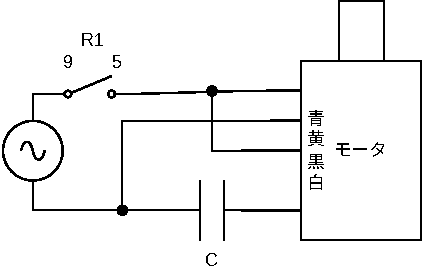
\includegraphics[width=0.5\textwidth]{sozai/8.pdf}
  \caption{コンベア1段目の配線図}
\end{figure}

\begin{figure}[H]
  \centering
  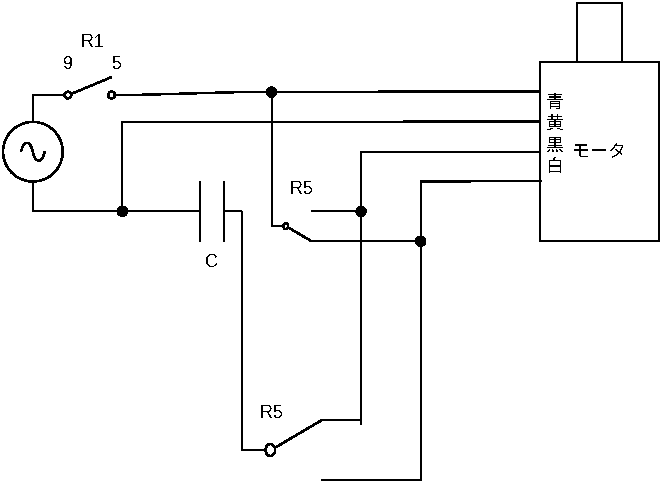
\includegraphics[width=0.5\textwidth]{sozai/9.pdf}
  \caption{コンベア2段目の配線図}
\end{figure}

\begin{figure}[H]
  \centering
  
\includegraphics[width=0.5\textwidth]{sozai/10.pdf}
  \caption{コンベア3目の配線図}
\end{figure}

そして,図3.6にPLCとの接続図を示す.PLCは電流+24Vで動作するため,
AC/DCコンバータが取り付けてある.各種センサからの出力信号がPLCのIN側(00 ch)
に入ってくるようになっている.PLCのOUT側(100 ch)には図3.3~3.5で示したように,
モーター起動および回転方向制御用の電磁リレーのコイル部(13,14番端子)とつながっている.

また,CPI1-Lでは出力点数が少ないため,追加拡張ユニットCPIW-16ERを使用している.
CPIW-16ERには16点の出力が追加される.追加拡張のアドレスは101 chおよび102 chである.
これを用いて,センサの信号(警告信号)を作る.101.01~101.07は拡張を用いてONとしておくことで
センサが機能するように配線が構成されている.

\begin{figure}[H]
  \centering
  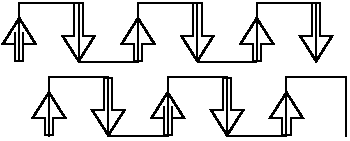
\includegraphics[width=0.5\textwidth]{sozai/11.pdf}
  \caption{PLC配線図}
\end{figure}

\section{実験方法}
本実験では,「PLCによるFA制御実験」を行う.以下に記載する課題3-1から3-3までを実施する.
なお,課題はラダープログラムを作成して動作確認を行うと共に,レポートにラダープログラム図を添付すること.

\subsubsection*{課題3-1 コンベア1段}
図表7のラダー図を基に,コンベア1段目の押しボタンスイッチを押すことで動作,
停止を繰り返すラダープログラムを作成せよ.

\subsubsection*{課題3-2 1秒のタイムラグ}
図表8のコンベアにおける前後方向のスイッチを行うラダー図を作成せよ.
ただし,課題3-1と同様に押しボタンスイッチを用いてタイムラグ1秒程度を設けること.
なお,タイムラグとしてTを利用する.

\begin{figure}[H]
  \centering
  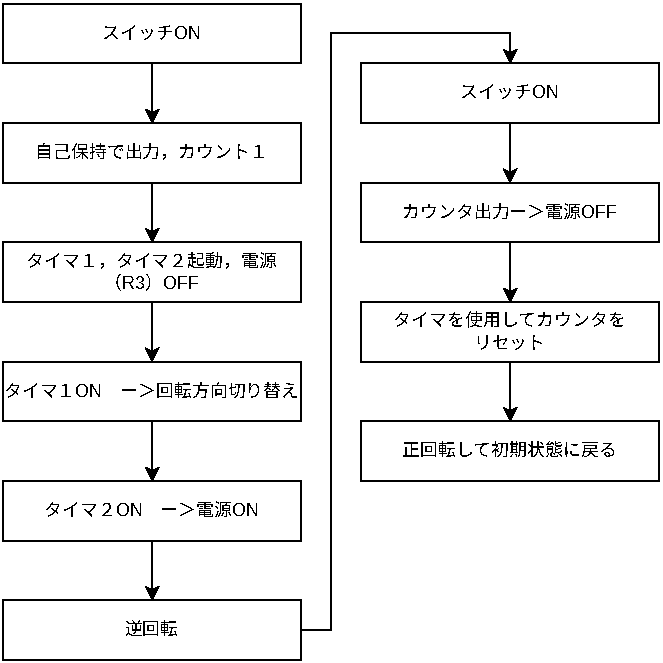
\includegraphics[width=0.5\textwidth]{sozai/12.pdf}
  \caption{課題3-2の流れ}
\end{figure}

\subsubsection*{課題3-3 最終課題}
非金属,非アルミ金属,アルミを振り分けるプログラムを作成せよ.
なお,コンベアのスイッチングに関して,タイムラグを設けること.
また,センサへの電力供給のため,図3.10に示すように101.01〜101.07はb接点を用いてONとしておくこと.

\section{実験結果及び考察}
本実験では,「PLCによるFA制御実験」を行う.以下に記載する課題3-1から3-3までを実施する.

\subsubsection*{課題3-1 コンベア1段}
図表7のラダー図を基に,コンベア1段目の押しボタンスイッチを押すことで動作,
停止を繰り返すラダープログラムを作成した

\begin{figure}[H]
  \centering
  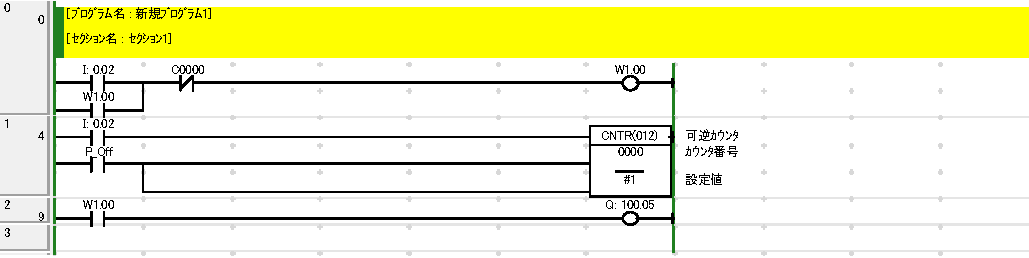
\includegraphics[scale=1]{sozai/3-1-crop.pdf}
  \caption{課題3-1}
\end{figure}
\begin{enumerate}
  \item 初期状態では, 押しボタンスイッチがOFFであり, コンベア1段は停止している.
  \item 押しボタンスイッチを押すと, 自己保持回路が形成され, コンベア1段が動作を開始する.
  \item コンベアが動作している間, カウンタ(CNTR)が作動し, 1回の動作サイクルごとにカウントアップされる.
  \item 再度押しボタンスイッチを押すと, 自己保持回路が解除され, コンベア1段が停止する.
  \item 上記の動作を繰り返すことで, 押しボタンスイッチの操作によってコンベア1段を動作および停止させることができる.
  \item カウンタの状態を監視することで, 動作サイクル数を記録し, 必要に応じて出力制御やリセットを行うことが可能である.
\end{enumerate}

\subsubsection*{課題3-2 1秒のタイムラグ}
図表8のコンベアにおける前後方向のスイッチを行うラダー図を作成した.
ただし,課題3-1と同様に押しボタンスイッチを用いてタイムラグ1秒程度を設けた.
なお,タイムラグとしてTを利用する.

\begin{figure}[H]
  \centering
  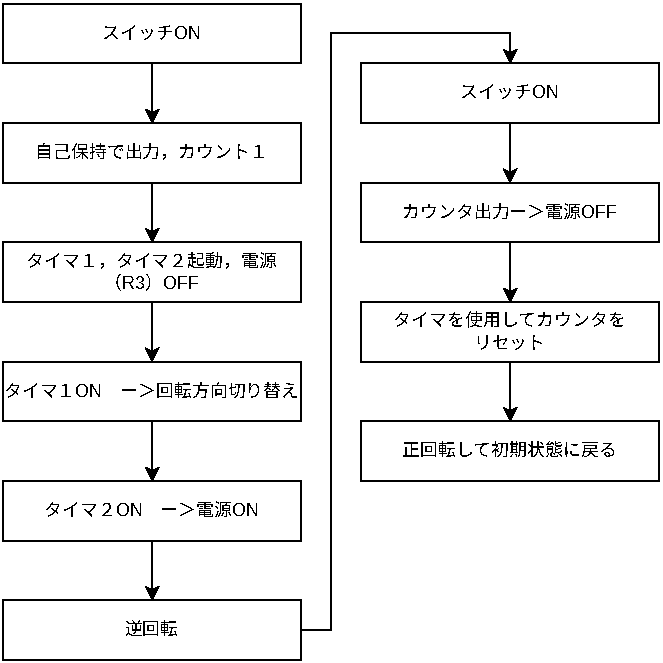
\includegraphics[width=0.5\textwidth]{sozai/12.pdf}
  \caption{課題3-2の流れ}
\end{figure}

\begin{figure}[H]
  \centering
  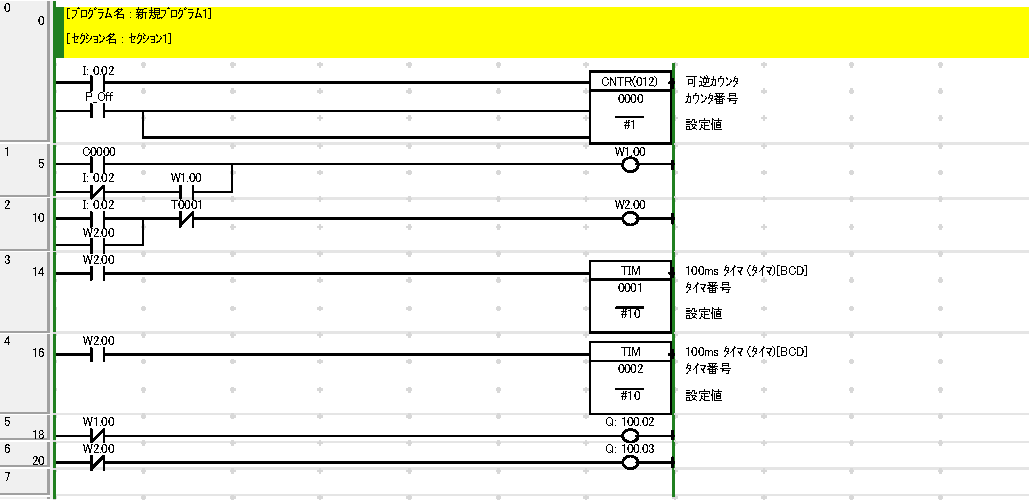
\includegraphics[scale=1]{sozai/3-2-crop.pdf}
  \caption{課題3-2}
\end{figure}

\begin{enumerate}
  \item 初期状態では, 押しボタンスイッチがOFFであり, コンベアは停止している.
  \item 押しボタンスイッチをONにすると, 自己保持回路が形成され, カウンタ(CNTR)が1カウントされる.
  \item カウンタが動作すると, タイマ(TIM000)およびタイマ(TIM001)が起動し, 設定時間のタイムラグが発生する.
  \item タイマ(TIM000)の設定時間が経過すると, コンベアが正転を開始する.
  \item カウンタの出力が切り替わることで, タイマ(TIM001)が動作し, 再びタイムラグを挟んでコンベアが逆転を開始する.
  \item スイッチを再び押すと, 自己保持回路が解除され, 全てのタイマおよびカウンタがリセットされる.
  \item この動作を繰り返すことで, 押しボタンスイッチの操作に応じてコンベアの前後方向切替を行うことが可能となる.
  \item タイムラグとしてタイマ(T)を利用し, 前後方向切替の際にスムーズな切替を実現している.
\end{enumerate}


\subsubsection*{課題3-3 最終課題}
非金属,非アルミ金属,アルミを振り分けるプログラムを作成した.
なお,コンベアのスイッチングに関して,タイムラグを設けた.
また,センサへの電力供給のため,図3.10に示すように101.01〜101.07はb接点を用いてONとしておく.
\begin{figure}[H]
  \centering
  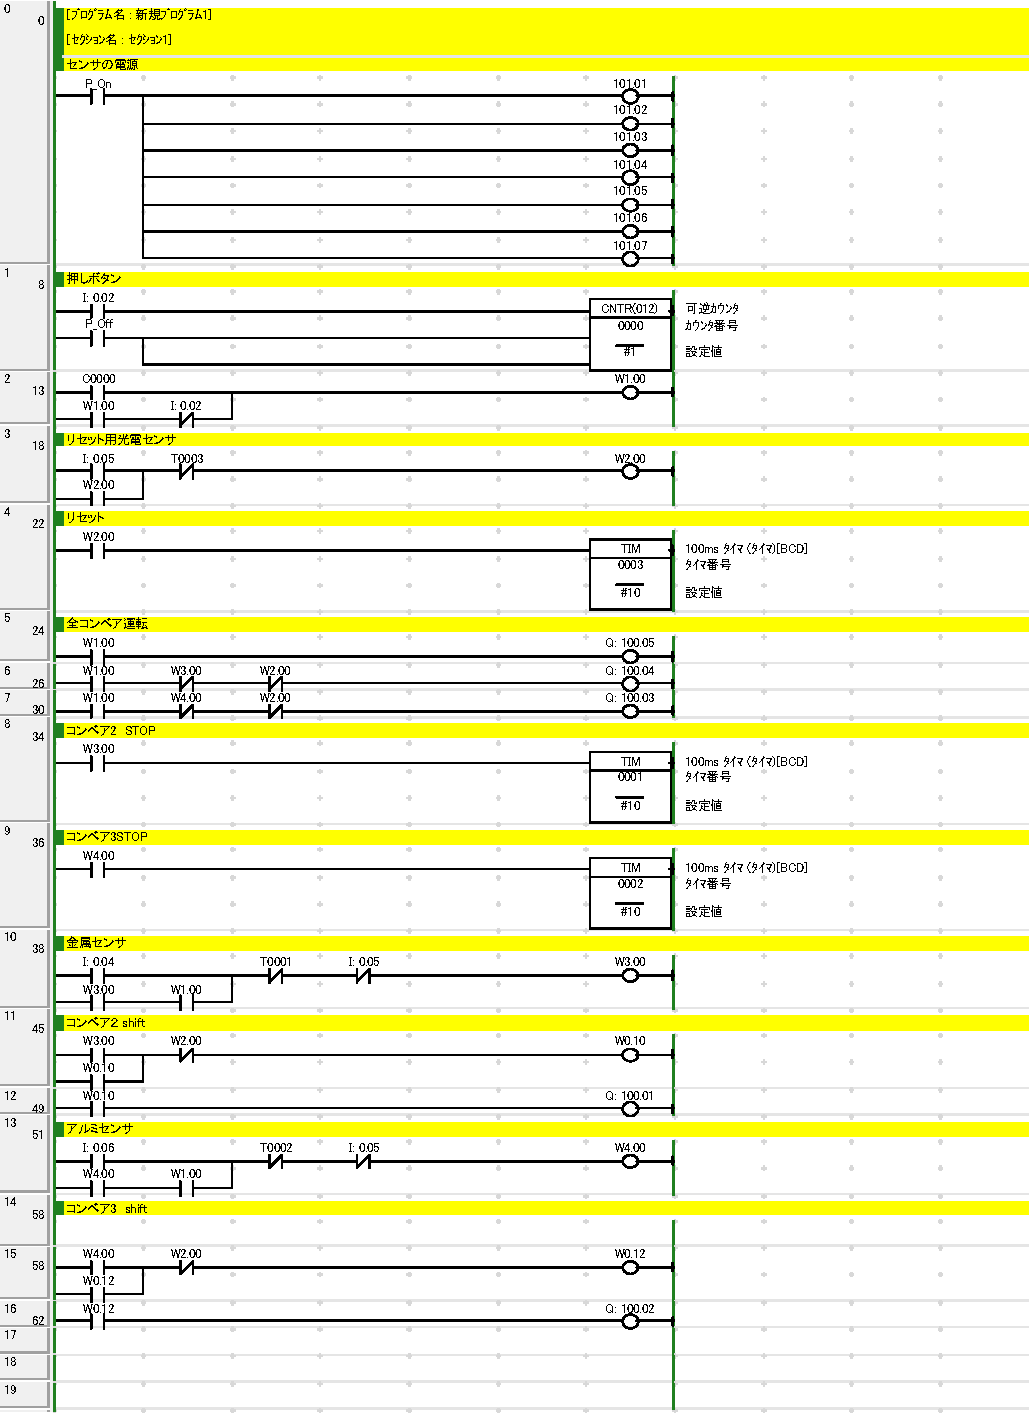
\includegraphics[scale=0.8]{sozai/3-3-crop.pdf}
  \caption{課題3-3}
\end{figure}

\begin{enumerate}
  \item 振り分け動作を開始するために,押しボタンスイッチ (I:0.02) をONすると,以下の動作が開始される:
        \begin{itemize}
          \item 自己保持回路が形成されることで,全体の回路が継続的に動作するようになる.
          \item 自己保持回路はC0000とW1.00の接点を利用し,押しボタンスイッチがOFFになっても回路が動作を継続する仕組み.
        \end{itemize}
  \item ワークがコンベアに搬送され,各センサを通過すると,以下の動作が個別に発生する:
        \begin{enumerate}
          \item 非金属検出 (センサI:0.04):
                \begin{itemize}
                  \item センサが信号を出力し,タイマ (T0001) が動作を開始する.
                  \item タイマ設定時間経過後,リレーW2.00が動作し,コンベア1が作動して非金属ワークを搬送する.
                \end{itemize}
          \item 非アルミ金属検出 (センサI:0.05):
                \begin{itemize}
                  \item センサが信号を出力し,タイマ (T0002) が動作を開始する.
                  \item タイマ設定時間経過後,リレーW3.00が動作し,コンベア2が作動して非アルミ金属ワークを搬送する.
                \end{itemize}
          \item アルミ検出 (センサI:0.06):
                \begin{itemize}
                  \item センサが信号を出力し,タイマ (T0003) が動作を開始する.
                  \item タイマ設定時間経過後,リレーW4.00が動作し,コンベア3が作動してアルミワークを搬送する.
                \end{itemize}
        \end{enumerate}
  \item タイムラグを利用した動作:
        \begin{itemize}
          \item タイムラグは,各コンベアの切り替え動作中の衝突や干渉を防ぐために設定されている.
          \item 各センサから信号を受け取ると対応するタイマが動作を開始し,設定された遅延時間が経過した後にリレーが動作してコンベアを起動する.
        \end{itemize}
  \item コンベア動作後,リセット用の光電センサ(I:0.07)が動作し,以下の処理を行う:
        \begin{itemize}
          \item 対応するタイマおよびリレーをリセットする.
          \item カウンタ (CNTR012) の値がインクリメントされ,処理されたワークの数を記録する.
        \end{itemize}
  \item 全ての処理が完了すると,押しボタンスイッチをOFFにすることで,自己保持回路が解除される:
        \begin{itemize}
          \item 自己保持が解除されることで,全てのリレー,タイマ,コンベアの動作が停止し,回路は初期状態に戻る.
        \end{itemize}
  \item 上記の動作が繰り返されることで,非金属,非アルミ金属,アルミの振り分けが継続的に行われる.
\end{enumerate}

